\documentclass{article}
\usepackage[utf8]{inputenc}
\usepackage{amsmath}
\usepackage{amssymb}
\usepackage{graphicx}
\usepackage{hyperref}
\usepackage[demo]{graphicx}

\title{Anode pad}
\author{fjwu }
\date{February 2020}

\begin{document}

\maketitle
\section{Abstract}
Microchannel-plate photomultipliers (MCP-PMT) are specialized vacuum photodetectors typically consisting of a photocathode, an amplification section consisting of several planes of glass micropores, and a segmented anode from which the amplified pulses are detected. \\
The spatial and temporal resolutions are determined by the conversion of the electron cascade pulse at the anode plane into a measurable signal, and also by the transport of that signal throughthe package wall to the diitizing electronics. 

\section{Introduction}

\subsection{cross-talk}

%\section{useful link}
%Capacitively coupled pickup in MCP-based photodetectors using a
%conductive metallic anode:\\
%\href{http://hep.uchicago.edu/cdf/frisch/papers//InsideOut_paper_aspublished.pdf}


\section{some figs (draft)}

\section{a. "parameters"}
The shape of one pad: regular/nose\\
The length of one pad:6 mm\\
radius of one laser spot:2\\
number of charges of one laser:1000\\
noise mean:1e-2 (Note: mean = 1e-2 * 1000 = 10)\\
noise variance:1e-3\\
number of simulation at one laser spot:3\\
number of laser pos:70\\
start pos:[-12,3]\\
end pos:[3,3]\\
(nose start:0.25\\
nose height ratio:0.2
sin height ratio:0.1)\\
\begin{figure}
\includegraphics[width=0.5\textwidth]{fig1.parameters.jpg}
\caption{this is the input.txt file, input parameters before running simulations}
\end{figure}

\section{b. pad pattern}
\begin{figure}
  \centering
  \begin{minipage}[b]{0.4\textwidth}
    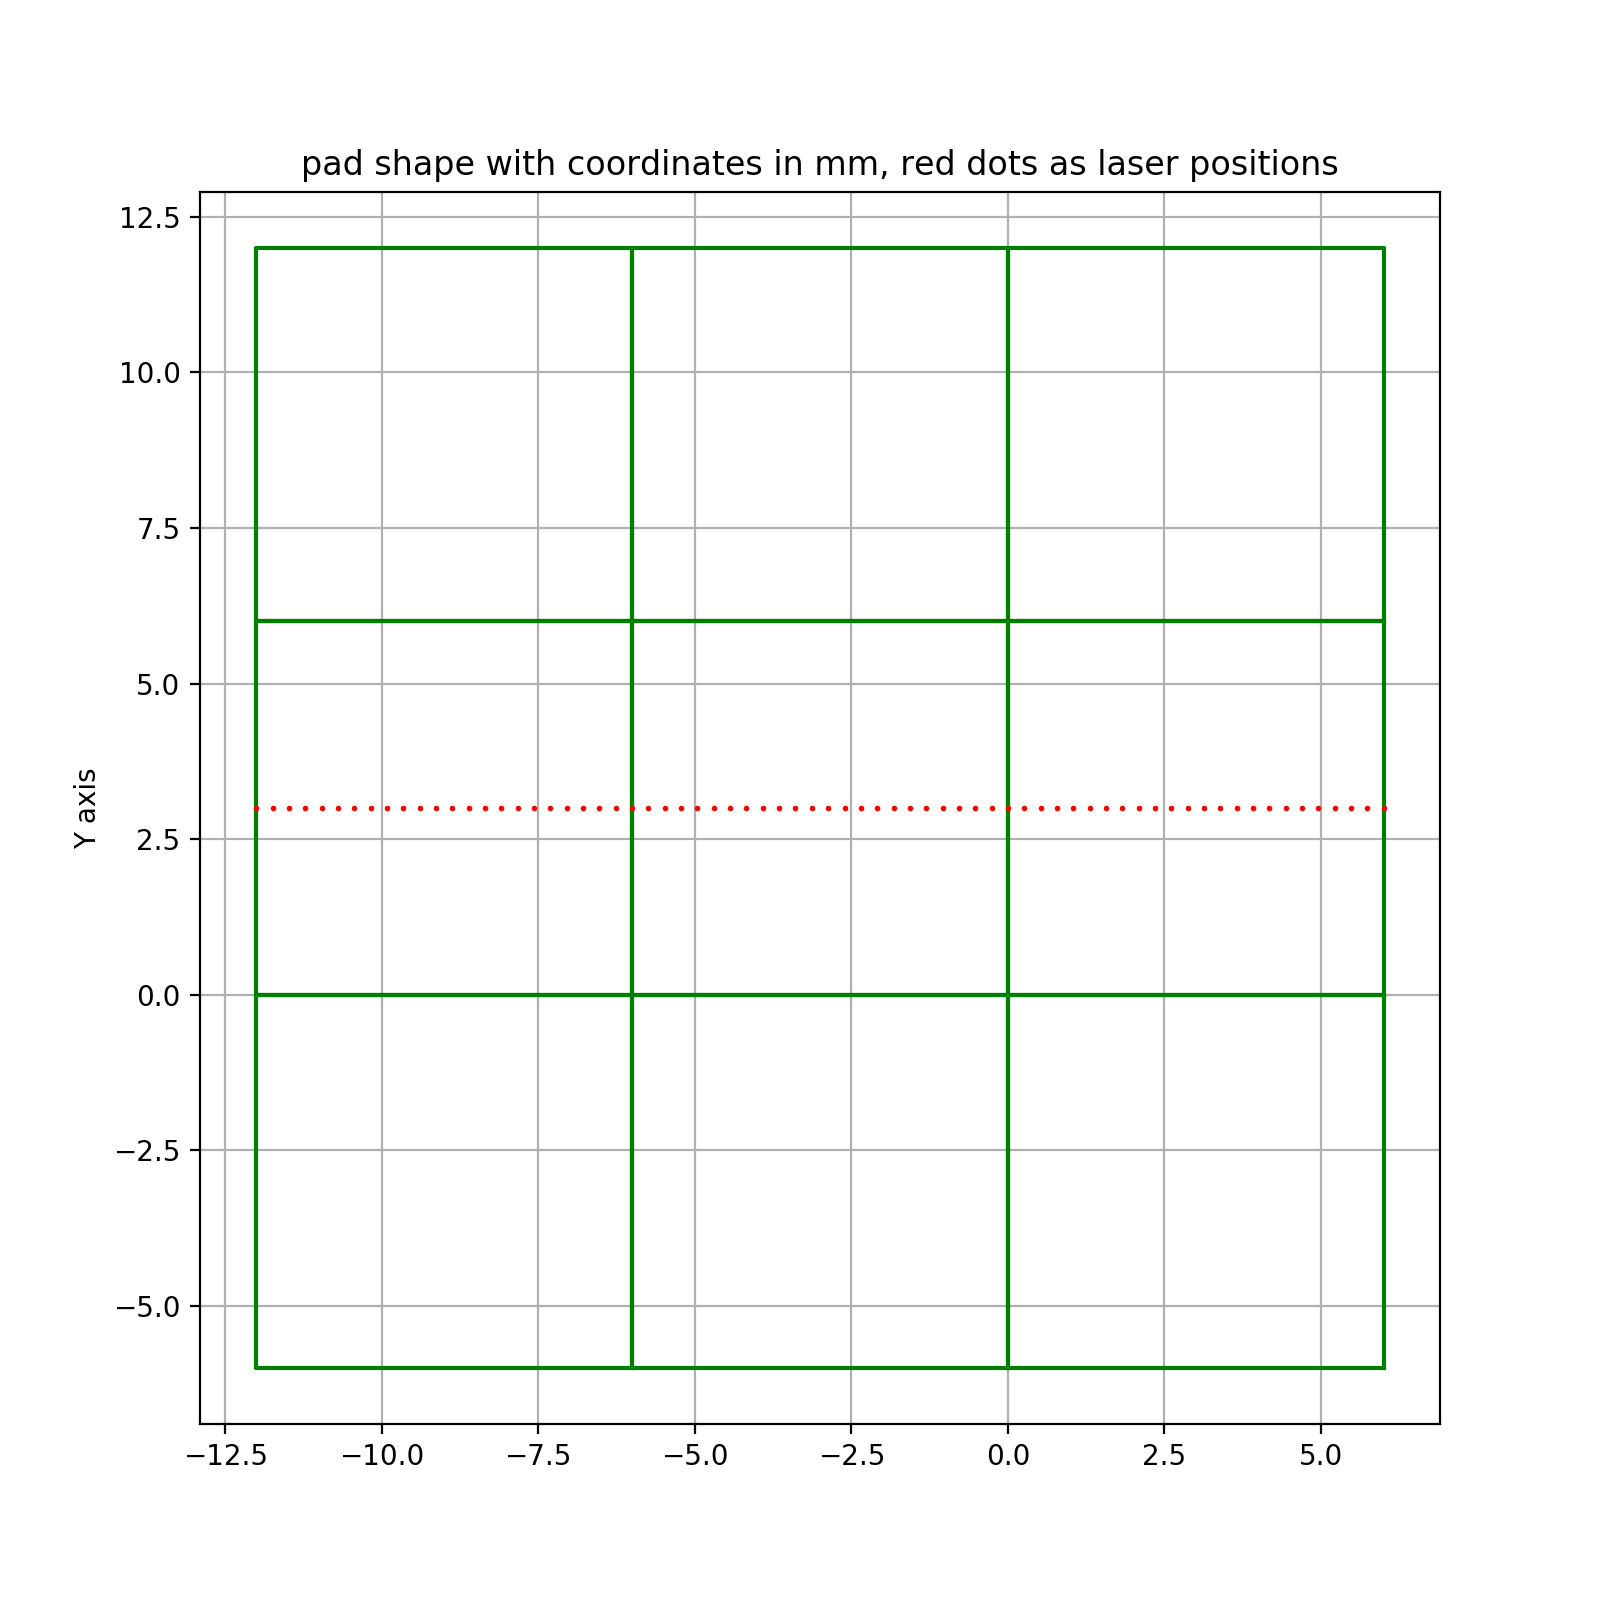
\includegraphics[width=\textwidth]{fig2_a rpad.png}
    \caption{9 square pads with width 6mm}
  \end{minipage}
  \hfill
  \begin{minipage}[b]{0.4\textwidth}
    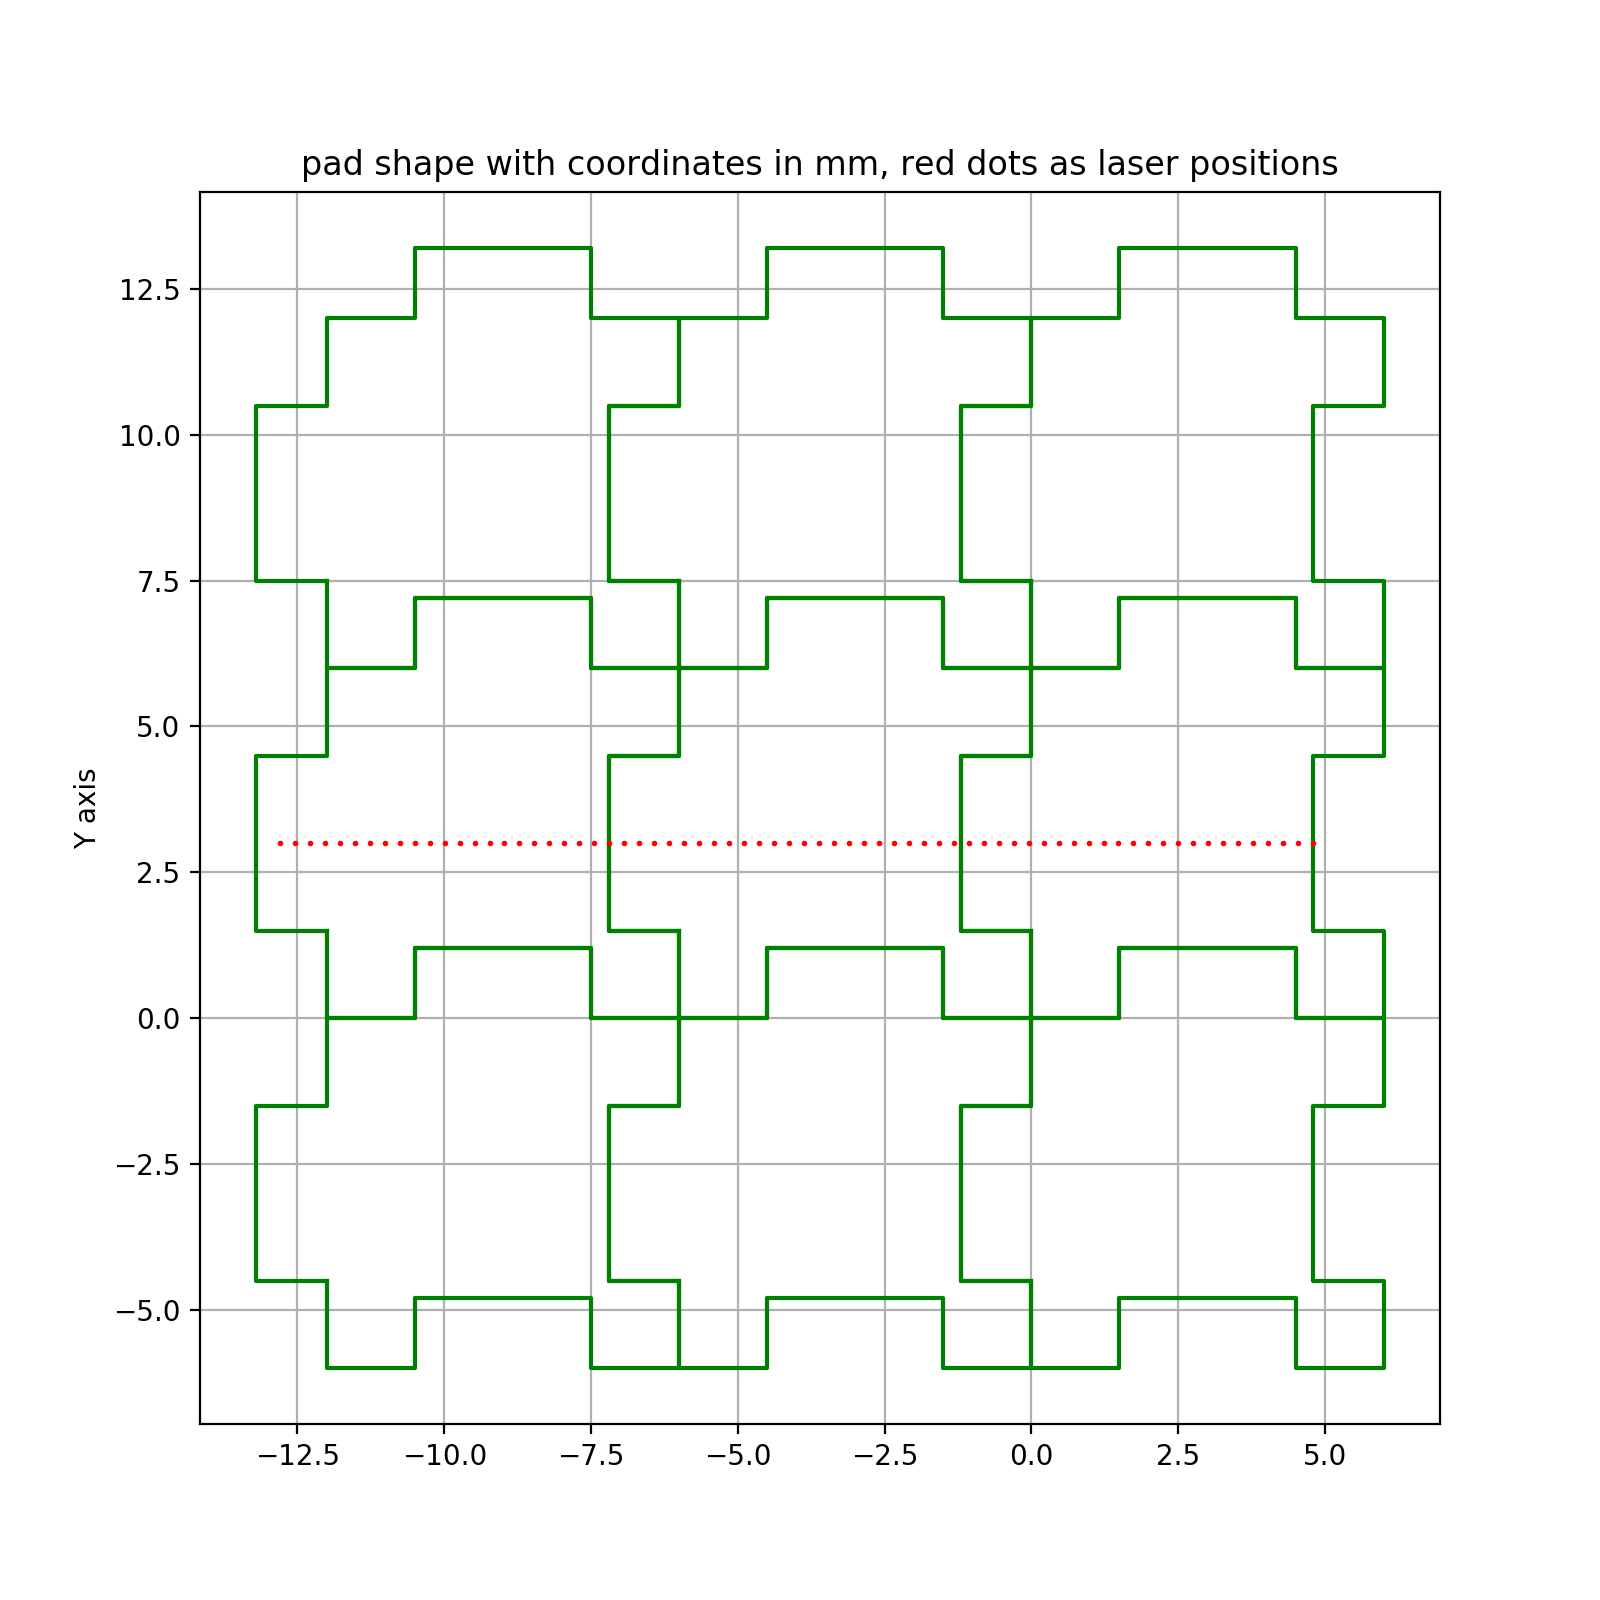
\includegraphics[width=\textwidth]{fig2_b.png}
    \caption{9 modified pads with width 6mm. extra rectangle is 3mm height, 1.2mm width}
  \end{minipage}
\end{figure}

\section{c. }
\begin{figure}
  \centering
  \begin{minipage}[b]{0.4\textwidth}
    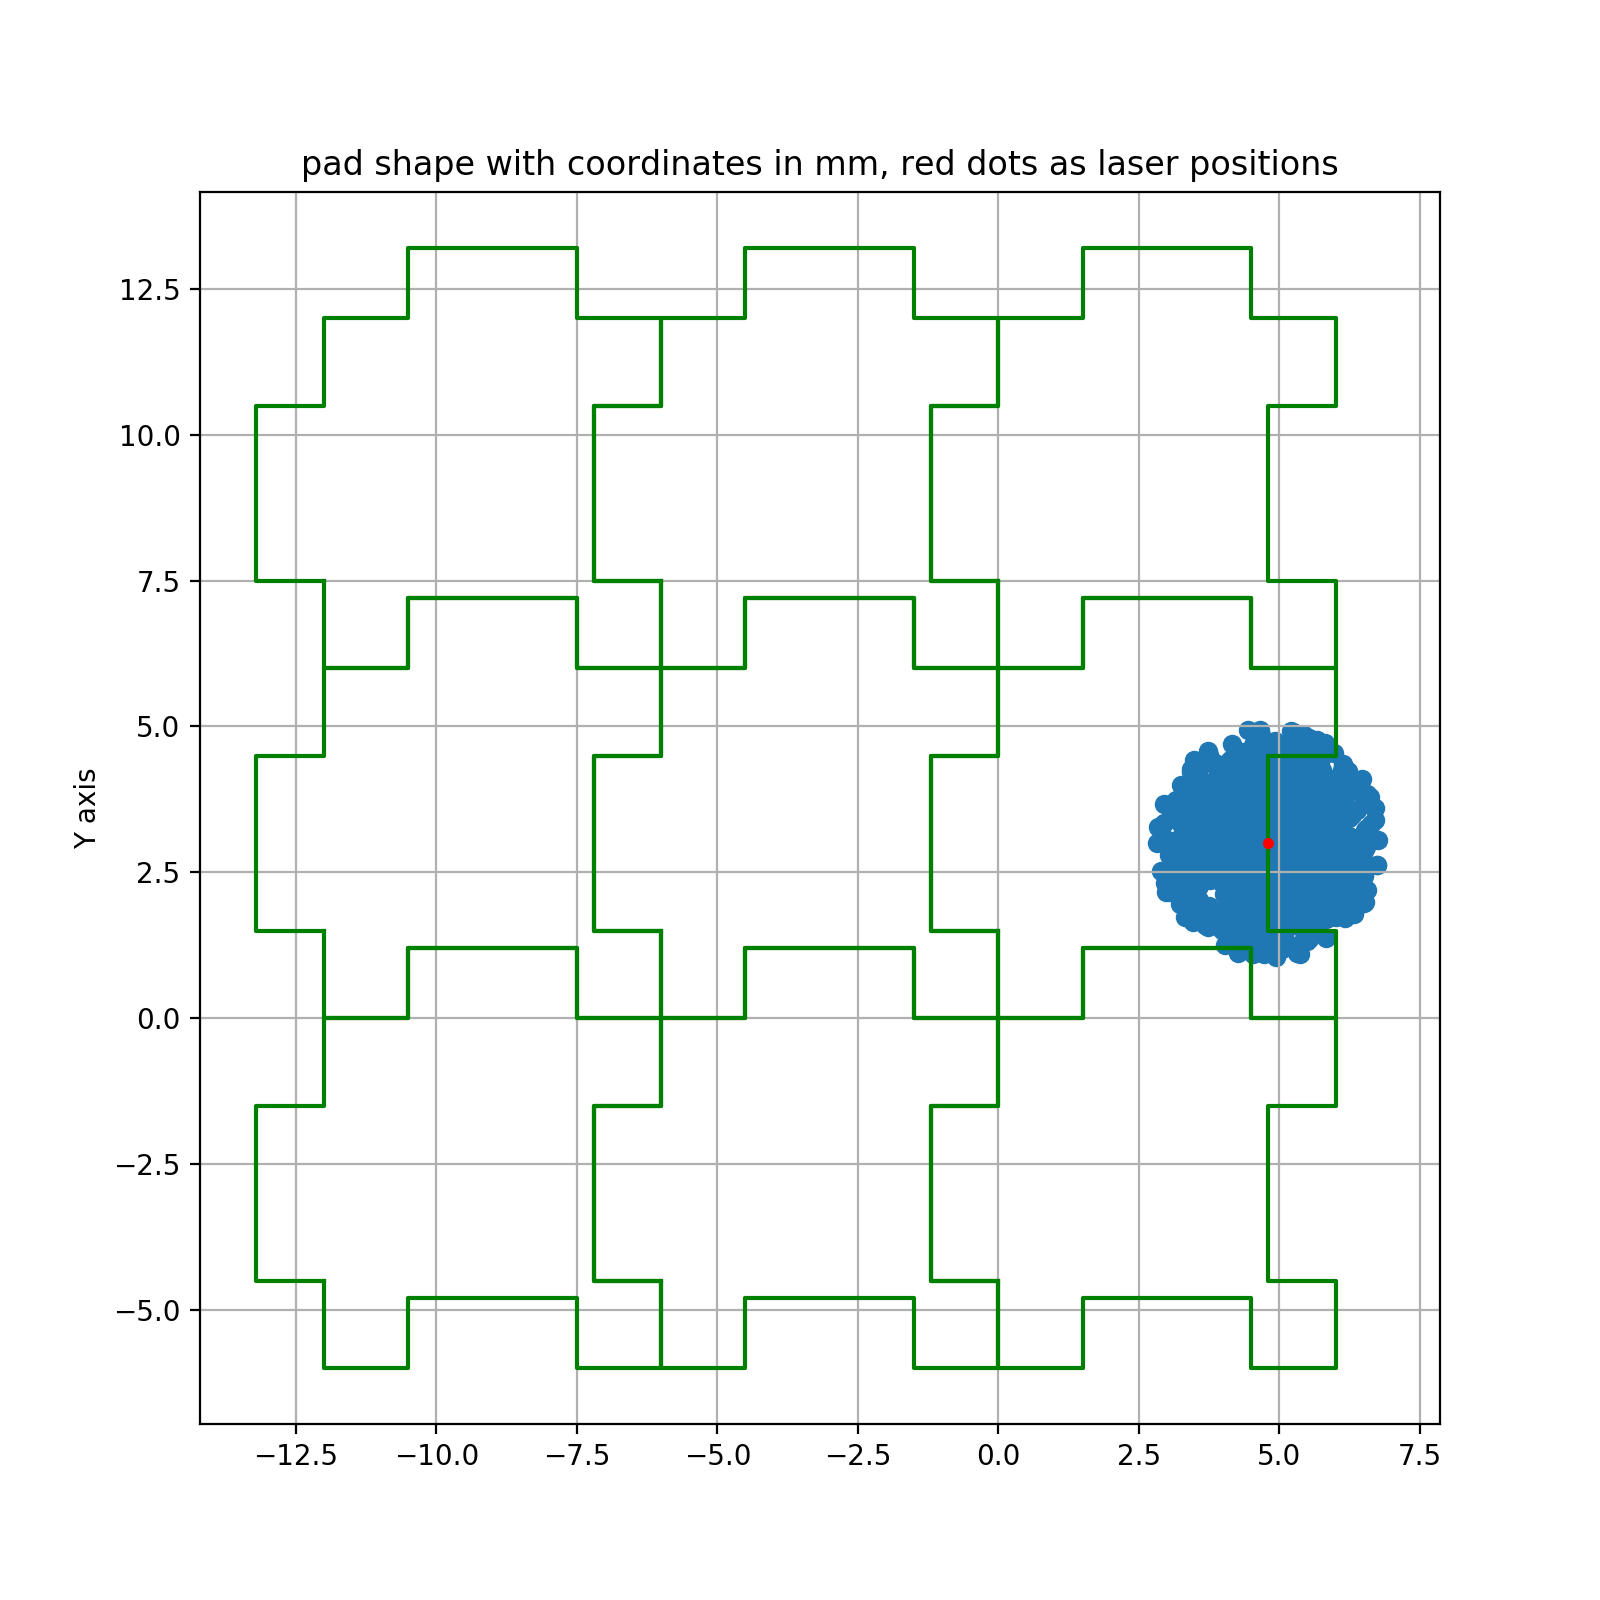
\includegraphics[width=\textwidth]{fig3_a.png}
    \caption{9 square pads with width 6mm}
  \end{minipage}
  \hfill
  \begin{minipage}[b]{0.4\textwidth}
    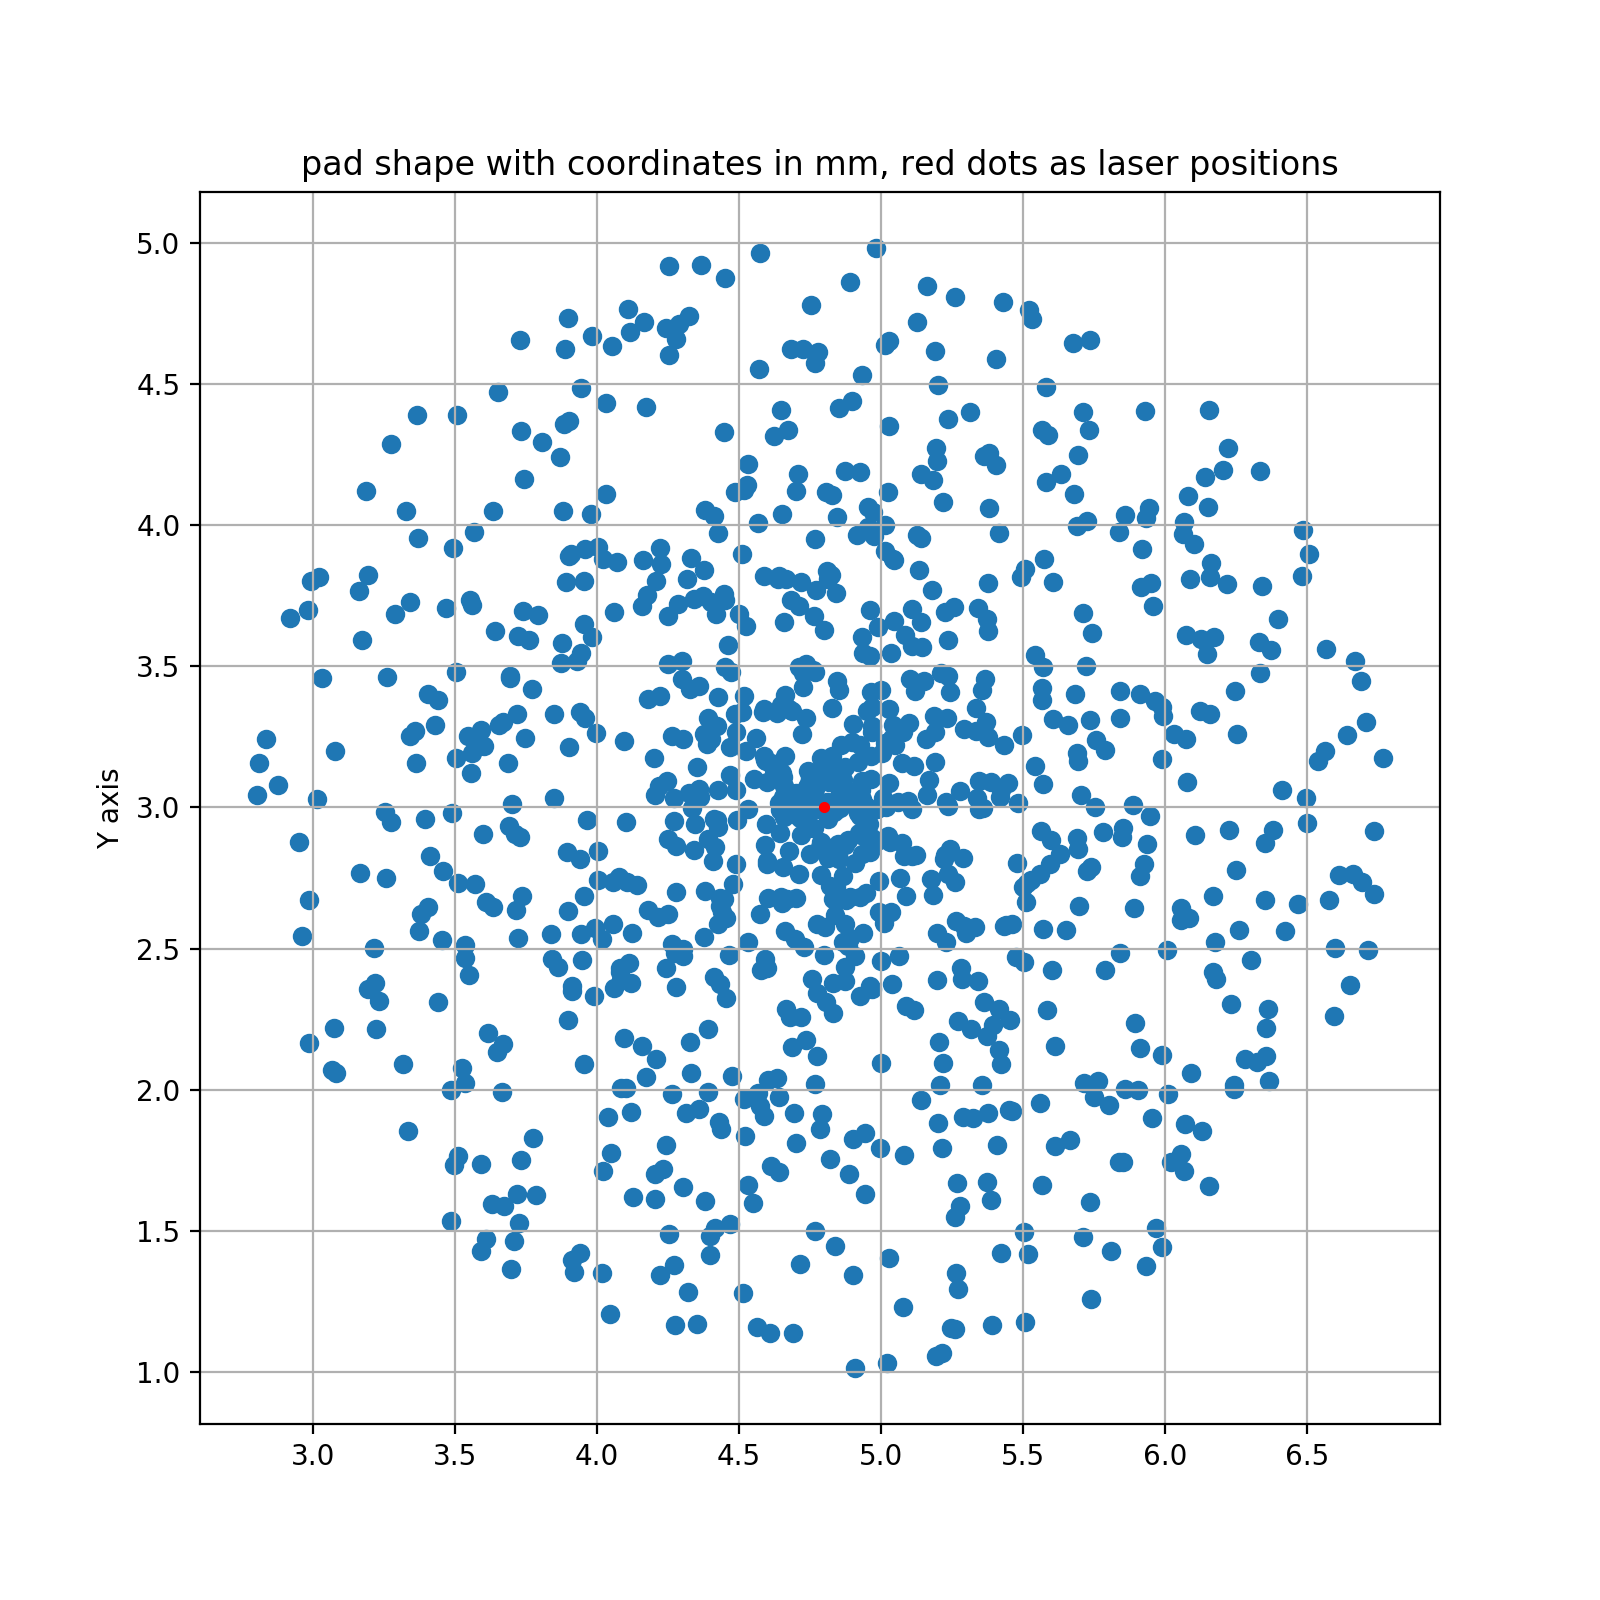
\includegraphics[width=\textwidth]{fig3_b.png}
    \caption{9 modified pads with width 6mm. extra rectangle is 3mm height, 1.2mm width}
  \end{minipage}
\end{figure}

\begin{figure}
  \centering
  \begin{minipage}[b]{0.4\textwidth}
    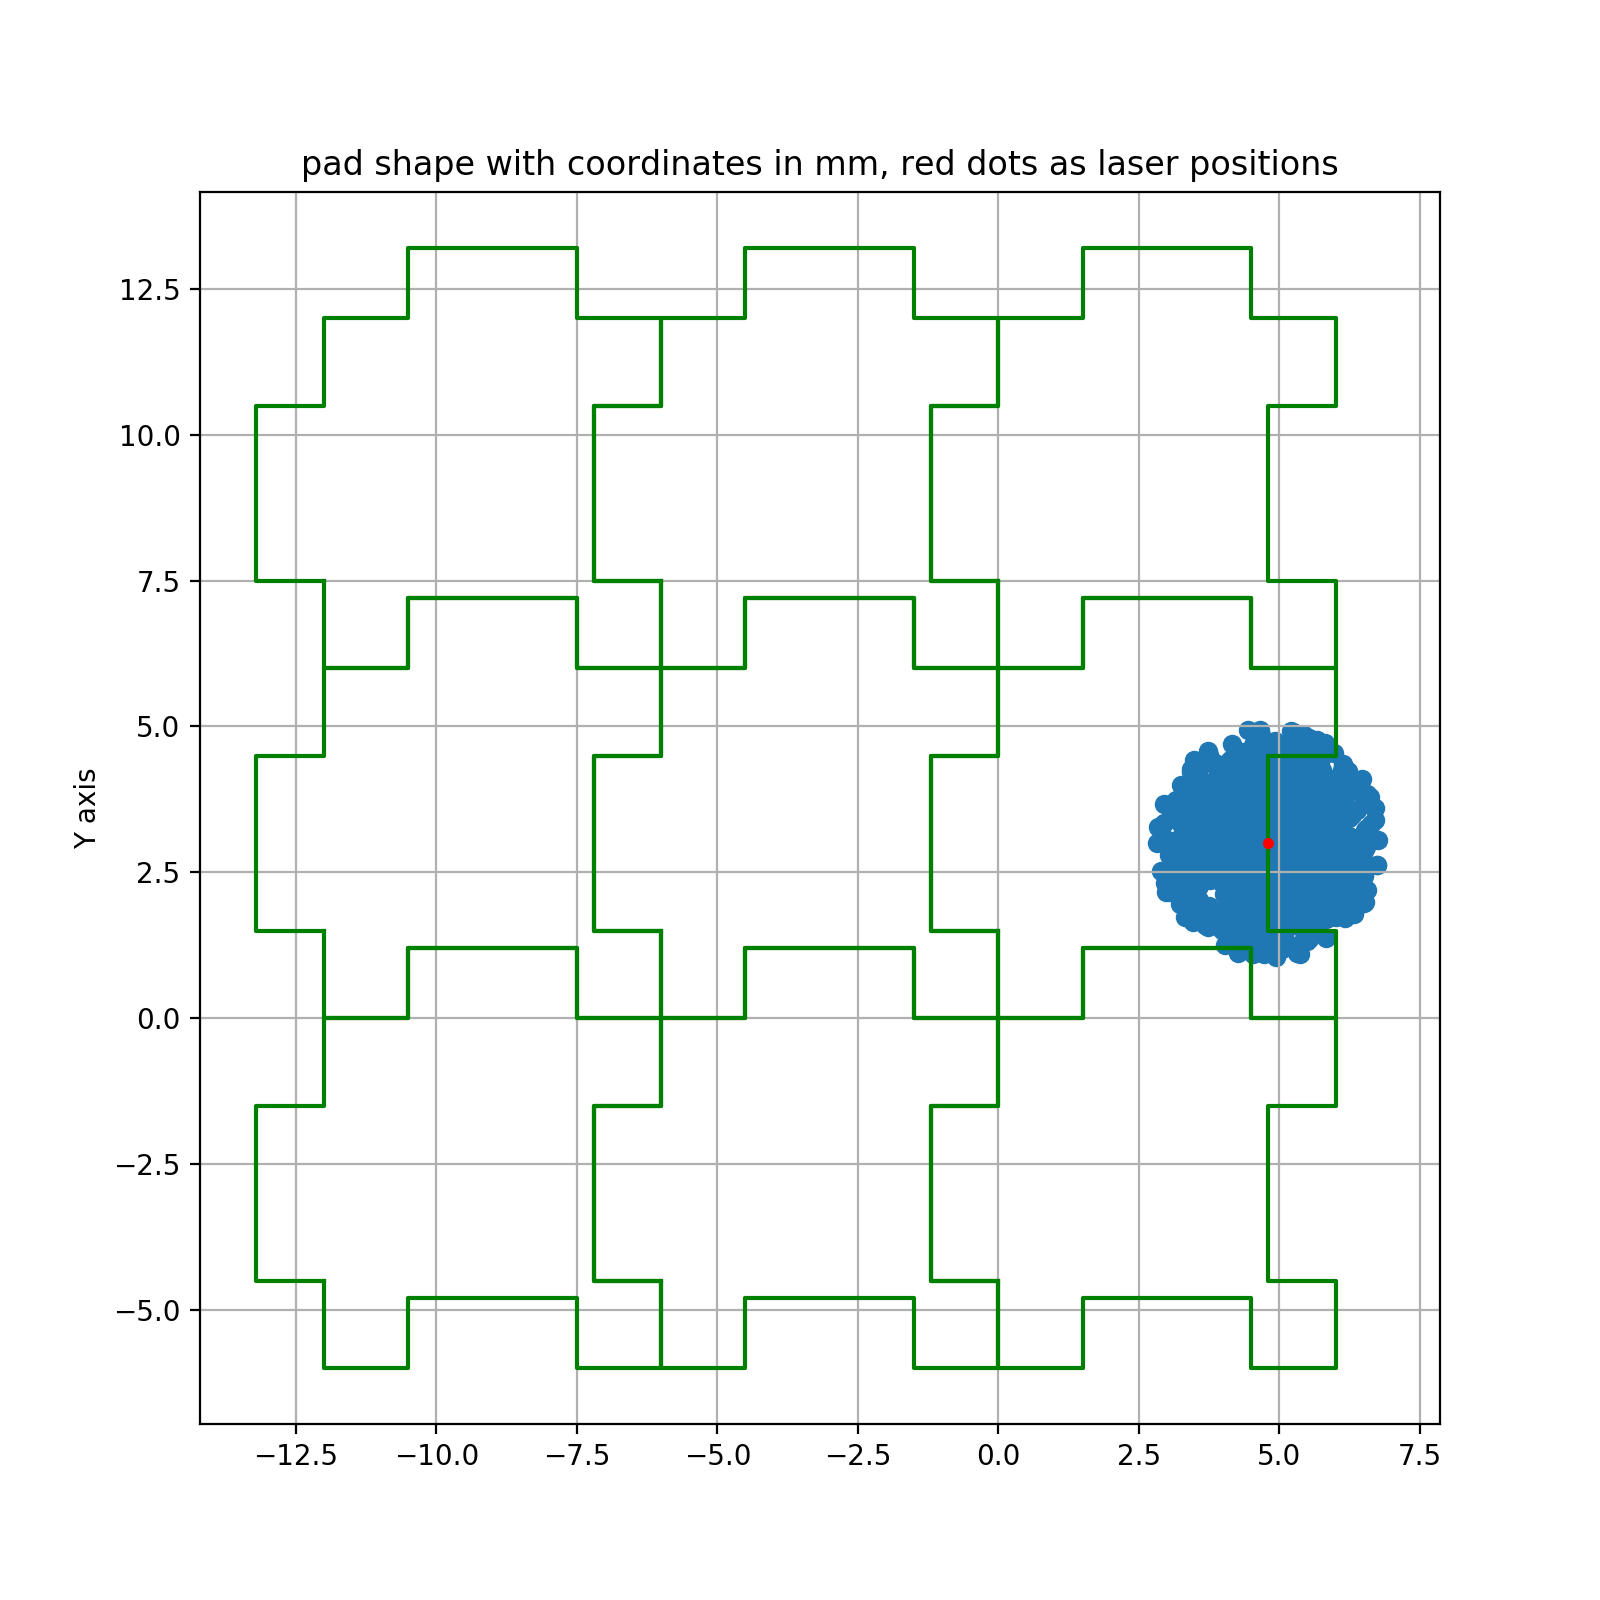
\includegraphics[width=\textwidth]{fig3_a.png}
    \caption{9 square pads with width 6mm}
  \end{minipage}
  \hfill
  \begin{minipage}[b]{0.4\textwidth}
    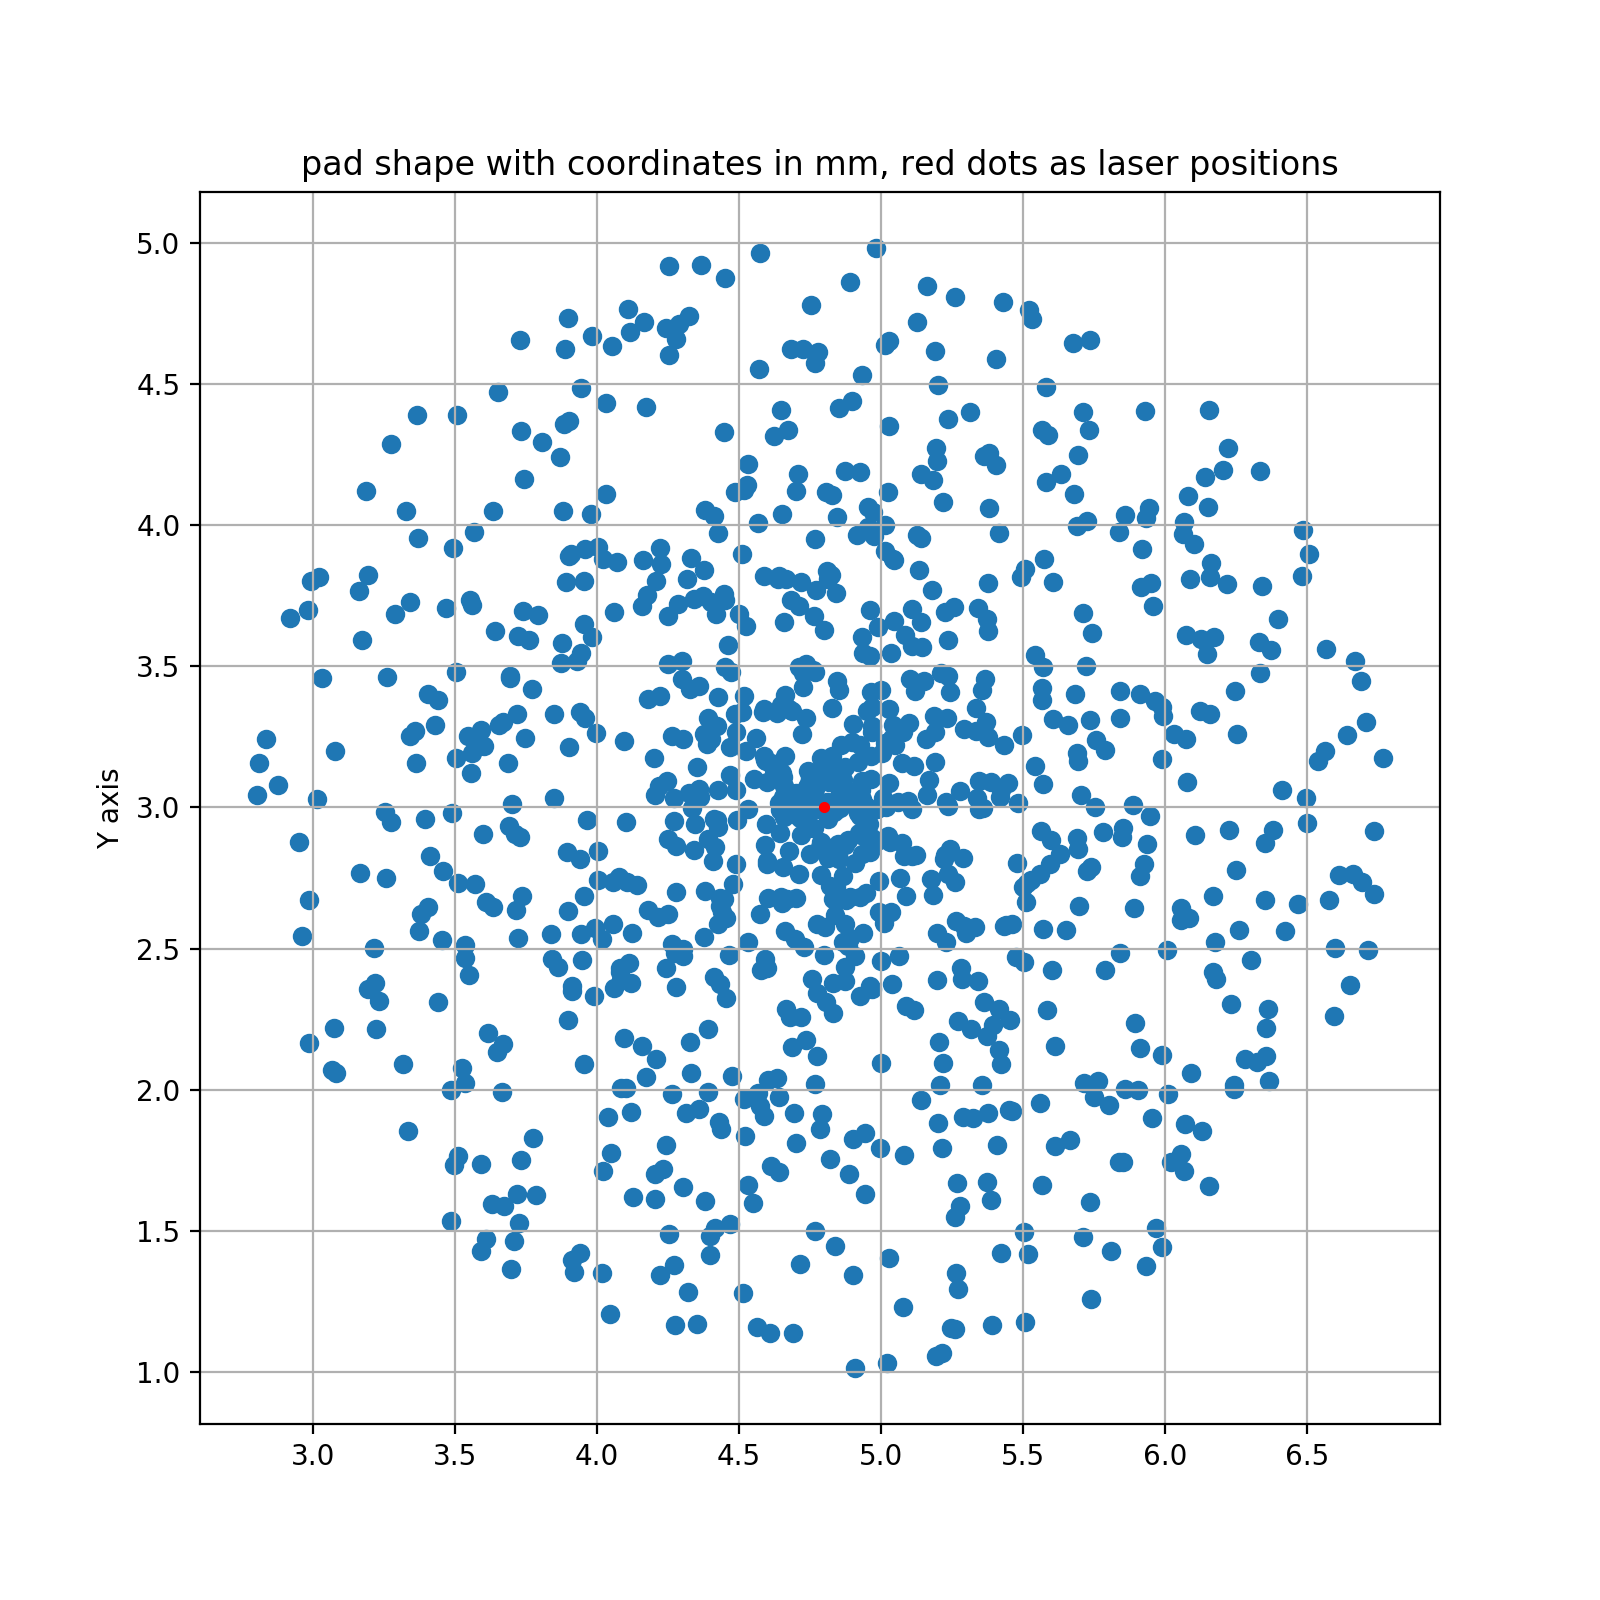
\includegraphics[width=\textwidth]{fig3_b.png}
    \caption{9 modified pads with width 6mm. extra rectangle is 3mm height, 1.2mm width}
  \end{minipage}
\end{figure}


\end{document}